%\documentclass{standalone}
%\usepackage{pgfplots}
%\begin{document}
%\pgfplotsset{
%	colormap={blackwhite}{[5pt]
%		rgb255(0pt)=(0,0,255); 
%		rgb255(100pt)=(0,255,255); 
%		rgb255(200pt)=(0,255,0); 
%		rgb255(300pt)=(255,255,0); 
%		rgb255(400pt)=(255,0,0)
%	},
%}
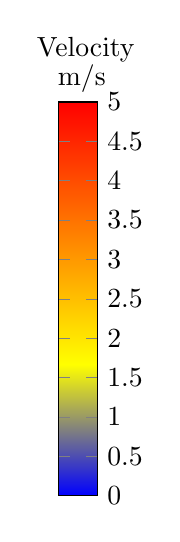
\begin{tikzpicture}
\node at (0.65,0.67) {Velocity};
\node at (0.6,0.3) {m/s};
\begin{axis}[
    hide axis,
    scale only axis,
    height=0pt,
    width=0pt,
    colorbar,
    point meta min=0,
    point meta max=5,
    colorbar style={
        height=5cm,
        ytick={0,0.5,1,...,5}
    }]
    \addplot [draw=none] coordinates {(0,0)};
\end{axis}
\end{tikzpicture}
%\end{document}
